\documentclass[oneside, 11pt, notitlepage, a4paper, numbers=noenddot]{scrartcl}

\usepackage{thisemi}
\usepackage{graphicx} 

\title { \begin{center}
    \textbf{WANNADRIVE?}
\end{center} 
Feasible Attack Paths and Effective Protection
Against Ransomware in Modern Vehicles}

\author{Johannes Winter}
\date  {Sommersemester 2021}

\begin{document}

\maketitle

\section{Einleitung}
In der Praxis hat sich jegliche Art von Cyber-Erpressungs-Malware auf IT-Systeme 
als sehr erfolgreich und lukrativ erwiesen. Jedes Jahr erzielen Erpresser so 
mehrere Milliarden US-Dollar Lösegeld und die Tendenz ist weiter steigend \cite[vgl.]{C..24.05.2020}. 
Durch die zunehmende Vernetzung und Digitalisierung entstehen immer größere 
potenzielle Angriffsziele, welche Opfer eines Ransomware-Angriffs werden können. 
Der eigene Computer, Unternehmens-IT-Systeme, SmartHome-Geräte oder IoT-Geräte – 
alle sind der Gefahr ausgesetzt. Nur ein vernetztes Gerät, welches täglich von 
Milliarden von Menschen benutzt wird, ist bis zum jetzigen Standpunkt noch kein 
Opfer von Ransomware-Angriffen geworden – das Auto. Gerade im Automobilbereich 
spielt das Thema Vernetzung und Digitalisierung eine sehr große Rolle und man 
strebt das Ziel eines vollständig vernetzten Straßenverkehrs an. Ein Auto muss 
mittlerweile mehr können als nur fahren und besteht aus sehr vielen softwaregesteuerten 
Komponenten. Diese wiederum erhöhen somit auch die potenzielle Angriffsfläche, vor 
allem für Ransomware. 
\newline
Der wissenschaftliche Artikel \cite{M.Wolf.2017} befasst sich mit diesem Thema und diskutiert 
einen solchen Angriff sowohl in der Theorie als auch in der Praxis und stellt Präventiv- 
als auch Gegenmaßnahmen dar. Der Inhalt dieses Artikels wird im Folgenden zusammengefasst 
wiedergegeben. 


\section{Erfolgsrezept Ransomware?}
Das Wort „Ransomware“ kommt von dem englischen Wort „ransom“ und 
bedeutet übersetzt „Lösegeld“. Dabei handelt es sich um Schadprogramme, 
meistens Erpressungssoftware oder Verschlüsselungstrojaner, mit denen ein 
Angreifer den Computer sperren und darauf befindliche Daten verschlüsseln 
kann. Erst nachdem das Opfer einer Lösegeldzahlung nachkommt, werden die 
Daten wieder freigegeben. 
\newline
Im Gegensatz zu fahrzeugbezogenen IT-Systemen, wo zum heutigen Stand wenig 
relevante Ransomware-Angriffe bekannt sind, werden in anderen IT-Bereichen 
bereits erfolgreich Ransomware-Attacken durchgeführt. Egal ob öffentliche und 
private Unternehmens-IT-Systeme, industrielle Steuerungssoftware, Websites, 
Smartphones oder sogar Live-TV-Sender – jede Art von IT-Systeme kann und ist 
bereits Opfer eines Ransomware-Angriffs gewesen. 
\newline
Aktuelle Studien schätzen den Anteil an infizierten, unaufgeforderten Emails auf 
bis zu 70$\%$. Im Jahr 2016 haben so Cyberkriminelle bereits rund 1 Milliarde US-Dollar 
erpresst. 2021 wird der Umsatz auf bis zu 20 Milliarden US-Dollar ansteigen \cite[vgl.]{C..24.05.2020}.  
\newline
Heutige Ransomware macht sich die zunehmende Digitalisierung und Konnektivität – aller 
Lebensbereiche – sowie der wachsenden Abhängigkeit von vernetzten IT-Systemen zunutze
und genau dies könnte schon bald auch moderne Fahrzeuge betreffen. 
Fahrzeuge werden nämlich immer:

\begin{enumerate}
    \item softwaregesteuerter (Vergrößerung der Anzahl potenzieller Angriffsziele)
    \item vernetzter (Vergrößerung der potenziellen Angriffsfläche)
    \item komplexer (Erhöhung der ausnutzbaren Sicherheitslücken)
\end{enumerate}
was die Anfälligkeit gegenüber Cybersicherheitsangriffen deutlich erhöht. 

In der Praxis wurden bereits alle bekannten Angriffsmuster hinsichtlich der 
Fahrzeugsicherheit (z.B. sicherheitskritische Fahrfunktionen wie Fahrzeuglenkung 
und -bremsung) erfolgreich demonstriert. Angriffe, welche sich jedoch auf die 
Fahrsicherheit des Fahrzeugs auswirken, noch nicht. Dies liegt daran, dass zur 
heutigen Zeit die häufigsten Fahrzeugsicherheitsangriffe immer noch dieselben sind 
wie früher: Fahrzeug-(Komponenten)Diebstahl, Kilometerzähler-Manipulation, (Chip-)Tuning 
und Herstellung gefälschter Teile. 
\newline
Gegen Diebstahl oder Phishing (ausnutzen unvorsichtigen Verhaltens) entwickelt die 
Automobilindustrie immer wieder neue und verschiedene Maßnahmen und Mechanismen. 
Ransomware hingegen wurde von den Sicherheitsingenieuren laut Autoren noch nicht wirklich 
in Angriff genommen. Dafür sehen die Autoren hauptsächlich zwei Gründe:
\begin{enumerate}
    \item Die Erstellung eines Fahrsicherheitsangriffs erfordert viel Zeit und Geld (viele 
    Personenmonate $\&$ $\>$100.000 Dollar Kosten), ermöglicht aber nur einen Angriff auf einen 
    bestimmten Fahrzeugtyp oder -klasse. Dies liegt daran, dass die meisten 
    Fahrzeug-IT-Architekturen und -Softwaren aufgrund ihrer Homogenität eine Übertragung 
    nicht so einfach ermöglichen.
    \item Der finanzielle Gewinn bei einem solchen Angriff bleibt bisher noch aus und oftmals 
    werden die Angreifer nur mit einem gewissen (akademischen) Ruhm belohnt. 
\end{enumerate}

Wie genau ein solcher Ransomware-Angriff in der Theorie und Praxis realisiert werden und 
aussehen könnte wird in den nächsten Kapiteln beschrieben.


\section{Fahrzeugbezogenen Ransomware in der Theorie}
Da es nach aktuellem Stand noch keine öffentlich bekannten fahrzeugbezogenen 
Ransomware-Angriffe gibt, lassen sich die Voraussetzungen für solch eine Cyber-Attacke 
nur grob abschätzen und von anderen Ransomware-Angriffen im IT-Bereich übertragen. Damit 
jedoch ein derartiger Cyber-Angriff tatsächlich umgesetzt werden kann, bedarf es der 
Notwendigkeit mindestens folgender fünf Bedingungen:

\begin{enumerate}
    \item Einen Ransomware-Malware-Client und eine Server-Software für die On-Board-Realisierung 
    der Cyber-Erpressung auf dem Zielfahrzeug zusammen mit der entsprechenden Fernsteuerung
    \item Ein anonymes Botnetz zur globalen Verteilung und Fernsteuerung der Ransomware-Fahrzeugclients
    \item Ein fahrzeuginterner Sicherheits-Exploit, meist zusammen mit einer Trojaner-Software zum 
    Erreichen und Infizieren einer angeschlossenen Fahrzeugeinheit, um den Ransomware-Malware-Client 
    zu installieren und auszuführen
    \item Eine bordeigene Sperr- oder Bricking-Aktion für eine kritische Fahrzeugkomponente, die 
    nicht (leicht) wiederhergestellt oder umgangen werden kann oder die sich keine lange Ausfalldauer 
    leisten kann - idealerweise kombiniert mit einem (geheimen) Entsperrbefehl, um die gesperrte 
    Fahrzeugkomponente nach Zahlung des Lösegelds freizugeben
    \item Ein anonymes Zahlungsschema zur Entgegennahme des Lösegelds und zum Schutz des Erpressers 
    vor Enttarnung und anschließenden rechtlichen Schritten
\end{enumerate}

Sind diese Voraussetzungen mindestens gegeben, dann könnte ein Ransomware-Angriff auf ein 
Fahrzeug wie folgt ablaufen:
\newline
\newline
Zu Beginn muss der Angreifer die Schadsoftware erstellen. Sobald eine funktionierende 
Ransomware programmiert wurde, muss diese auf die ausgewählten Erpressungs-Zielfahrzeuge 
mittels einer Ransom"-ware-Steuerungssoftware verteilt werden. Im besten Fall geschieht dies 
mittels eines anonymen Botnetzes, welches beispielsweise auf der TOR-Technologie 
\footnote{„The Onion Router“ – Verschlüsselung der Daten in mehreren Schichten, um anonymes 
surfen zu ermöglichen} basieren könnte. 
\newline
Hat die Software das Zielfahrzeug erreicht, muss dieses infiziert werden. Das kann direkt oder  
indirekt erfolgen.
\newline
Eine direkte Infizierung könnte beispielsweise über eine USB-Schnittstelle oder Ladeschnittstelle 
realisiert werden. Eine indirekte Infizierung hingegen würde sich eine sekundäre Sicherheitslücke zu Nutze 
machen und über eine Zwischenkomponente versuchen, die Software auf das Fahrzeug zu laden. 
Das kann z.B. eine infizierte Website sein, auf welche das Fahrzeug zugreifet.
\newline
Wenn dieses Vorgehen erfolgreich ist und die Software das Fahrzeug erreicht hat, wird 
der integrierte primäre Sicherheits-Exploit des Fahrzeuges genutzt, um den Ransomware-Client auf 
einer zentralen, gut vernetzten Einheit im Fahrzeug zu installieren und auszuführen. Diese Einheit 
könnte z.B. das Infotainment-System sein, welche dann als Host für weitere Aktionen missbraucht 
wird.
\newline
Je nachdem, mit welchem Vorgehen die Erpresser das Auto manipulieren wollen, kann der 
Ransomware-Client entweder eine Online-Verbindung zurück zum Erpresser aufbauen, um weitere 
Daten und/oder Befehle zu erhalten oder den Weg direkt über die fahrzeuginternen Bussysteme nutzen. 
Über diese könnte die Schadsoftware mit kritischen Steuergeräten (z.B. Motorsteuerung) 
kommunizieren, um somit die geplante Sperraktion durchzuführen. 
\newline
Ist dieses Vorhaben gelungen, muss nur noch die Erpressermeldung mit den 
nötigen Details zur anonymen Bezahlung auf einem Bildschirm im Fahrzeug angezeigt werden. 
Im Falle, dass das Opfer das geforderte Lösegeld tatsächlich bezahlt, würde die Ransomware 
erneut das Bot-Netzwerk kontaktieren, um den (geheimen) Entsperrbefehl zu erhalten, damit  
das Fahrzeug wieder freigeben werden kann.


\section{Fahrzeugbezogenen Ransomware in der Praxis}
In Kapitel 3 wurde besprochen, was eine fahrzeugbezogene Ransomware-Attacke 
für nötige Voraussetzungen haben muss und wie diese in der Theorie ablaufen 
könnte. 
In diesem Kapitel soll es nun darum gehen, wie dieses Vorhaben in der Praxis 
aussehen und ablaufen könnte. Dabei wird auf die Abläufe \textbf{„Erstellen einer 
fahrzeugbezogenen Ransomware-Malware“, „Verbreitung der Fahrzeug-Ransomware-Malware“, 
„Infizierung des Zielfahrzeugs“, „Erpressung im Zielfahrzeug“ und „Ablauf der 
Lösegeldzahlung und Freigabe des Zielfahrzeugs“} genauer drauf eingegangen.

\subsection{Erstellen einer fahrzeugbezogenen Ransomware}
Wie bereits in Kapitel 2 erwähnt ist fast jedes IT-System angreifbar 
für Ransomware und viele davon wurden bereits erfolgreich infiziert. 
Der dadurch entstandene lukrative Markt hat dazu geführt, dass es mittlerweile 
fertige Ransomware-Baukästen und Ransomware-as-a-Service (RaaS)-Angebote gibt. 
Solche Kits enthalten den notwendigen Malware-Kontrollserver und eine fertige 
Schnittstelle zu einen anonymen Bezahlungsmittel und Traffic-Anonymisierer. 
\newline
Einige solcher Ransomware-Kits bieten darüber hinaus auch gängige Sicherheits-Exploits 
für die Verteilung der Ransomware und Zielfunktion zur Verfügung. In einigen Fällen 
kann ein solches Kit sogar sogenannte „Zero-Day-Exploits“ zur Integration in die 
Software bereitstellen. Dabei handelt es sich um Sicherheitslücken, welche dem 
Entwickler/Unternehmen der betroffenen Einheit noch nicht bekannt ist. Dadurch 
kann diese Schwachstelle noch individueller und leistungsfähiger ausgenutzt werden.
\newline
Selbst der gewünschten Erpressungsmechanismus kann bei solchen Baukästen ausgewählt 
werden. Egal ob Verschlüsseln der Daten, Sperren wichtiger Komponenten oder mögliches 
Freigeben sicherheitskritischer Daten – der Erpresser hat fast unbegrenzte Möglichkeiten, 
den für sich optimalen Erpressungsmechanismus auszuwählen.
\newline
So kann mittels dieser Kits ein Angreifer innerhalb kurzer Zeit und mit wenigen Klicks 
eine funktionierende Ransomware mit allen notwendigen Komponenten erstellen.
\newline
Bis jetzt ist es jedoch noch nicht möglich, mit Hilfe solcher Baukästen Schadsoftware 
für fahrzeugbezogene IT-Systeme zu erstellen, da die meisten Kits hauptsächlich für 
Microsoft Windows-Betriebssysteme ausgelegt sind. Laut Autoren ist es jedoch nur eine 
Frage der Zeit und finanziellen Attraktivität, bis solche Erstellungssoftwares auch für 
\textit{automotive Linux} oder \textit{AUTOSAR-OS} programmiert werden. 

\subsection{Verbreitung der fahrzeugbezogenen Ransomware}
Um die Verteilung der Ransomware auf eine große Anzahl an Fahrzeuge zu verbreiten 
und dabei sowohl effizient als auch anonym zu bleiben, bietet sich ein TOR-basiertes 
Botnetz an. Ein solches Botnetz kann in der nötigen Größe von mindestens 400.000 
„Bot-Clients“ schon für 1000\$ pro Woche angemietet werden. 
\newline
Zwar erreichen solche Botnetze das Fahrzeug nicht direkt, können aber zumindest 
indirekt Fahrzeuge infizieren, indem sie ein Host-System befallen und missbrauchen, 
welches über einen digitalen Kommunikationskanal zum Fahrzeug verfügt. Solche Host-Systeme 
könnten sein:

\begin{itemize}
    \item Websites, die vom Fahrzeug abgerufen werden (z. B. Drive-by-Downloads, die über 
    die bordeigene Infotainment-Einheit oder über versteckte Machine-to-Machine-Website-Anfragen 
    abgerufen werden)
    \item Nachrichten, die vom Fahrzeug abgerufen und interpretiert werden (z. B. E-Mails, SMS, 
    digitale Messenger, E-Call, DAB+ Radio)
    \item Persönliche Geräte, die mit dem Fahrzeug verbunden sind (z. B. Smartphones, digitaler 
    Speicher, Navigation, OBD-Plugins)
    \item Jedes mit dem Fahrzeug verbundene OEM- oder Lieferanten-Backend (z. B. für FOTA-Updates, 
    Ferndiagnose, Cloud-Dienste)
    \item Jedes mit dem Fahrzeug verbundene Backend von Drittanbietern (z. B. für Versicherung, 
    Telematik, Maut, Logistik, Leasing)
    \item Alle Geräte von Drittanbietern, die mit dem Fahrzeug verbunden sind (z. B. Anhänger, 
    Fahrzeugperipherie oder Anbaugeräte, Elektroladestation, Werkstattgeräte, digitaler 
    Fahrtenschreiber)
    \item Verkehrsinfrastrukturen (z. B. Verkehrsmanagementsysteme, Baustellenzugangskontrollgeräte, 
    Mautsysteme, V2X)
\end{itemize}
	
Je nachdem, wie leistungsfähig die erstellte Ransomware ist, kann die Verbreitung der 
Schadsoftware entweder aktiv oder passiv erfolgen. Eine aktive Verbreitung ist möglich, 
wenn die Software eine gewisse Leistungsfähigkeit und einen sekundären Infektionsmechanismus 
besitzt. Ist die Leistungsfähigkeit jedoch nicht gegeben, dann muss die Verbreitung passiv 
erfolgen, d.h. über das entsprechende Botnetzwerk.   

\subsection{Infizierung des Zielfahrzeugs}
Hat die Ransomware nun eine digitale Fahrzeugschnittstelle erreicht, muss der 
Client nur noch auf der entsprechend leistungsfähigen und gut vernetzten elektronischen 
Steuereinheit (ECU) im Fahrzeug installiert und ausgeführt werden.
\newline 
Mehrere Studien bzw. Forschungsarbeiten haben bereits bewiesen, dass fahrzeuginterne 
Sicherheitslücken existieren, welche durch eine Ransomware missbraucht werden könnten. 
In einer dieser gelang es den Sicherheitsexperten Zugriff auf die interne Software zu 
erlangen. Von Ärgernissen wie unkontrolliertem Hupen bis hin zu ernsthaften Gefahren 
wie dem Bremsen des Prius bei hohen Geschwindigkeiten, die Servolenkung abschalteten, 
das GPS und Tachometer fälschen -  mit den Befehlen, welche sie von ihren Laptops aus 
schickten, war fast alles möglich, um das Auto in eine gefährliche Fahrsituation zu 
bringen. (QUELLE)
\newline
Sowohl die zunehmende Digitalisierung, die zunehmende Vernetzung als auch die zunehmende 
Homogenisierung und Standardisierung im Fahrzeug tragen dazu bei, dass die Skalierbarkeit 
der Angriffe erhöht wird, da so mehr einheitliche Fahrzeugsicherheitsschwachstellen 
entstehen. Diese wären:

\begin{itemize}
    \item Schwachstelle im USB-Anschluss des Fahrzeug-Infotainment-Systems
    \item Schwachstellen im OBD-Port für den Zugriff auf alle Busse im Fahrzeug
    \item CD/DVD-Player-Schwachstelle am Fahrzeug-Infotainment-System
    \item Bluetooth-Pufferüberlauf-Schwachstelle bei Fahrzeug-Infotainment-Einheit
    \item Zellulare Verwundbarkeit an der zentralen Fahrzeugkommunikationseinheit
    \item Wi-Fi-Schwachstelle am Ladesystem für Elektrofahrzeuge
    \item Remote-Schwachstelle am Telematik-Steuergerät (TCU) des Nachrüstmarktes
    \item Schwachstellen in mobilen Fahrzeug-Apps für den Zugriff auf Fahrzeuginterna
    \item Ausnutzung des Wi-Fi-Stacks durch Google Project Zero
\end{itemize}
	

\subsection{Erpressung im Zielfahrzeug}
Wurde die Ransomware erfolgreich installiert und ausgeführt, kann die 
eigentliche Geiselnahme beginnen. In diesem Fall ist die Geisel sinnbildlich:

\begin{itemize}
    \item eine gesperrte oder "gemauerte" kritische Fahrzeugkomponente, die nicht 
    (einfach) wiederhergestellt oder umgangen werden kann oder die sich keine lange 
    Ausfalldauer leisten kann
    \item die Beschlagnahmung oder das Durchsickern kritischer Fahrzeugdaten, die nicht 
    (einfach) wiederhergestellt werden können oder die einen erheblichen Schaden 
    verursachen würden, wenn sie öffentlich zugänglich würden
    \item irgendetwas anderes, um das Opfer zur Zahlung des Lösegelds zu zwingen 
    (z.B. reine Behauptung, es sei etwas gesperrt worden)
\end{itemize}

Sobald einmal der Zugriff gelungen ist, hat der Angreifer schier unendliche 
Möglichkeiten, um seine Epressungsaktion durchzuführen. In Abbildung \ref{fig:Erpressung} sind 
mögliche Systemkomponenten dargestellt, welche sich zum Bricken, Sperren oder 
Leaken anbieten würden.
\newline

\begin{figure}[htbp!]
    \centering
    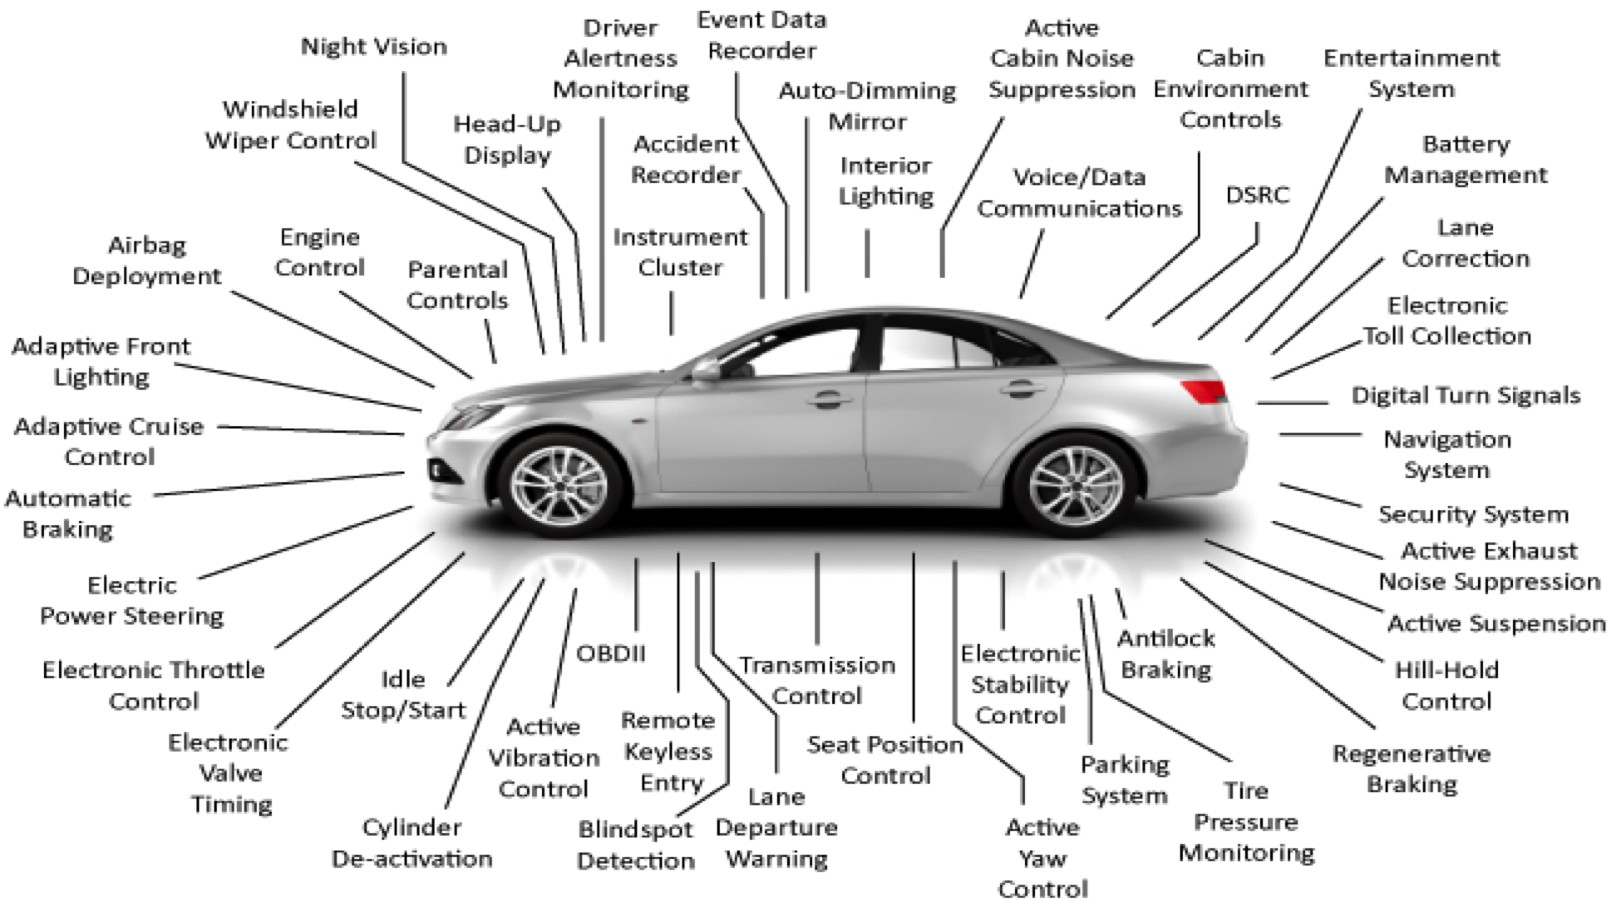
\includegraphics[width=0.94\textwidth]{Images/Diagnostic-Scanning-1.jpg}
    \caption{Mögliche Systemkomponenten, welche durch eine Ransomware missbraucht werden könnten}
    \label{fig:Erpressung}
\end{figure}

Abbildung \ref{fig:Erpressung} macht deutlich, dass es in heutigen Autos zahlreiche Systeme gibt, 
auf denen man ein Cyber-Angriff durchführen kann. Sei es das Blockieren wichtiger 
Steuergerätsfunktionen oder kryptografischer Anmeldeinformationen, das Verschlüsseln 
von kritischen Daten, das Freigeben kritischer (interner) Daten im Fahrzeug, das 
Manipulieren von Sensor- oder Servodaten oder das Manipulieren/Zerstören kritischer 
Fahrzeugkomponenten – ein Angreifer hat schier unendliche Möglichkeiten. 
\newline
Sobald die Geiselnahme durchgeführt (oder vorgetäuscht) wurde, wird die Ransomware 
für das Opfer sichtbar. Eine solche Erpressungsmeldung erklärt in der Regel die eigentliche 
Erpressungssituation klar und deutlich und bietet sehr detaillierte Hilfe und Informationen, 
wie das geforderte Lösegeld zu zahlen ist. Zur Demonstration haben die Autoren eine 
solche Meldung erstellt, welche in Abbildung \ref{fig:WannaDrive} zu sehen ist. 
\newline

\begin{figure}[htbp!]
    \centering
    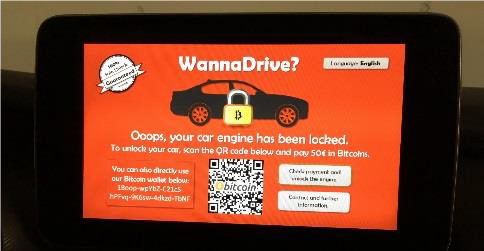
\includegraphics[width=0.94\textwidth]{Images/WannaDrive.png}
    \caption{Beispielhafte Erpressungsmeldung mit Zahlungsinformationen}
    \label{fig:WannaDrive}
\end{figure}

\subsection{Ablauf der Lösegeldzahlung und Freigabe des Zielfahrzeugs}
\input{Sections/4.5. Ablauf der Lösegeldzahlung und Freigabe des Zielfahrzeugs.tex}

\section{Präventivmaßnahmen gegen fahrzeugbezogene Ransomware}
Wie in den vorherigen Kapiteln dargestellt, gibt es unzählige Möglichkeiten, ein 
Fahrzeug mittels Ransomware zu attackieren. Dementsprechend gibt es auch keine 
Allumfassende Schutzmaßnahme, welche vor allem schützt. Vielmehr benötigt man ein 
ganzheitliches Security-Engineering-Konzept, welches einen vollständigen, systematischen 
und mehrschichtigen Schutzansatz verfolgt. 
Dieses Konzept umfasst:

\begin{itemize}
    \item Das komplettes Fahrzeugsystem (d.h. vom einzelnen Steuergerät bis 
    zum angeschlossenen Cloud-Backend)
    \item den gesamten Fahrzeuglebenszyklus (d.h. von der ersten Anforderungsanalyse 
    bis zur Ausmusterung des Fahrzeugs)
    \item die komplette Fahrzeugorganisation (d.h. von den Sicherheitsprozessen 
    bis zur Security Governance)
\end{itemize}

Dies wiederum gestaltet sich als schwierig und kostspielig im Gegensatz zu 
klassischen IT-Systemen, da Fahrzeuge deutlich mehr Angriffspunkte haben, 
keine effektive Sicherung von Daten oder Funktionen durchführen können, in den 
meisten Fällen keine regelmäßigen Sicherheitsupdates erhalten und nur eine einfache 
Firewall besitzen.

\subsection{Absicherung des gesamten Fahrzeugsystems}
Da man davon ausgehen muss, dass ein Angreifer das Zielfahrzeug nach der 
schwächsten Komponente absuchen würde, muss bei der Absicherung das gesamte 
Fahrzeug betrachtet werden. Das heißt, dass man von jedem einzelnen Steuergerät 
bis hin zu angeschlossenen Backend-Diensten alles betrachtet werden muss. 
\newline
Des Weiteren ist es von Vorteil, gleichzeitig mehrere Verteidigungslinien zu haben, 
da man davon ausgehen muss, dass eine der Schutzmaßnahmen geschwächt wird oder ausfällt.
\newline
Einen Schutzansatz nach dem „Singel Point of Failure“ Prinzip, sollte man definitiv 
vermeiden. Dieser geht davon aus, dass eine einzige Komponente (z.B. Firewall) das 
gesamte sichere interne Fahrzeugnetzwerk von einem unsicheren, externen Netzwerk isoliert. 
Sollte ein Angreifer in dieser Komponente eine Schwachstelle entdecken hätte das zur 
Folge, dass auf einmal alle Fahrzeuge des betroffenen Typs komplett kompromittiert würden. 
\newline
Um ein solches Szenario zu verhindern und entgegenzuwirken muss der Angriffspfad so 
oft wie möglich durchbrochen werden. Dazu empfehlen die Autoren folgende Maßnahmen:

\begin{itemize}
    \item Fahrzeug-Cybersicherheit Intelligenz $\&$ Forschung
    \item Klassische Unternehmenssicherheit für alle Fahrzeug-IT-Infrastrukturen
    \item Starke Backend-Zugriffskontrolle für alle fahrzeugbezogenen Assets, Schnittstellen 
    und Funktionalitäten
    \item Vollständiger Schutz der Fahrzeugschnittstellen
    \item Sichere Fahrzeug-E/E-Architektur
    \item System zur Erkennung und Verhinderung von Eindringlingen in das Fahrzeug
    \item Fahrzeuginterne Firewall
    \item Verfahren zur Reaktion auf Vorfälle
\end{itemize}

\subsection{Absicherung des gesamten Fahrzeuglebenszyklus}
Neben der Absicherung des gesamten Fahrzeugsystems muss auch der 
gesamte Fahrzeuglebenszyklus betrachtet werden, der sich 
vom Start der Entwicklung bis zur Ausmusterung des Fahrzeugs erstreckt. Dies garantiert, 
dass man auf die sich ständig ändernden Sicherheitsanforderungen schnellstmöglich 
reagieren kann und somit neu entdeckte Schwachstellen beheben und neu entwickelte 
Sicherheitsansätze einbringen kann.
\newline
Ein solcher kontinuierlicher Lebenszyklus hat auch einige zusätzliche technische 
und organisatorische Implikationen. Die gesamte Entwicklungshardware, alle 
Werkzeugketten und zumindest ein Teil der beteiligten Experten müssen bis zur endgültigen 
Ausmusterung verfügbar bleiben, was für schwere Nutzfahrzeuge einen Zeitraum
von bis zu 20 Jahren bedeutet.

\subsection{Absicherung der gesamten Fahrzeugorganisation}
Die letzte Komponente im mehrschichtigem Schutzansatz behandelt die Absicherung 
der gesamten Fahrzeugorganisation und erfordert eine tiefgreifende, bereichsübergreifende 
Integration und ein starkes Engagement der gesamten Organisation, einschließlich 
dediziertem Budget, Mitarbeitern und Befugnissen. 
\newline
Eine gut aufgestellte Sicherheitsorganisation kann die Sicherheitsrisiken durch die 
Verringerung der Komplexität reduzieren, einen guten Systemüberblick bieten und für 
eine ordnungsgemäße Verwaltung aller sicherheitskritischen Funktionen und der 
entsprechenden Berechtigungsnachweise sorgen. 


\section{Maßnahmen gegen fahrzeugbezogene Ransomware}
\input{Sections/6. Maßnahmen gegen fahrzeugbezogene Ransomware.tex}

\section{Schlusswort}
Aktuell sind Ransomware-Angriffe auf Fahrzeuge noch Theorie, doch schon in naher 
Zukunft kann sich dies ändern. Aufgrund der zunehmenden Digitalisierung und Konnektivität 
von Autos bieten sich den Angreifern viele Angriffsflächen, welche, wenn die Automobilindustrie 
ihren Securityansatz nicht um den Aspekt Ransomware erweitert, schon bald rigoros ausgenutzt 
werden könnten. Hinter Ransomware-Angriffen steckt ein überzeugendes Geschäftsmodell und wenn 
man dadurch viel Geld verdienen kann, wird es auf kurze oder lange Sicht Personen geben, die 
sich dies zum Vorteil machen möchten.
\newline
Ziele werden weniger Privatpersonen werden, sondern eher Nutzfahrzeuge und große Fahrzeugflotten, 
da diese meist auf ihre Fahrzeuge angewiesen sind und sich keine lange Ausfalldauer leisten können.
\newline
Es ist unabdingbar, dass sich die Automobilindustrie auf Ransomware-Angriffe vorbereiten muss, 
indem sie die Schutzfunktionen in gleichem Tempo auf Fahrzeuge ausweitet, sich mit ganzheitlichen, 
mehrschichtigen Schutzmaßnahmen auf die Bedrohung vorbereitet, aber auch die Fähigkeit, mit 
aktualisierten Abwehrmaßnahmen und Reaktionen auf Angriffe zu reagieren, auf Fahrzeuge ausweitet.
\newline
Dieses Paper gibt nur einen kleinen Einblick in das Thema fahrzeugbezogene Ransomware-Angriffe. 
Aufgrund der begrenzten Seitenanzahl konnten nicht alle Aspekte erwähnt oder tiefgründiger diskutiert 
werden aber das Themengebiet bietet enorm viel Potential, in welchem tiefgründigere Forschungen 
getätigt werden können, um somit der Sicherheit für Autos beizutragen. 


\bibliographystyle{IEEEtran}
\bibliography{Quellen/Quellenverzeichnis_Citavi_texfile}

\end{document}
